\chapter{Repair}
Some heuristic could generate an invalid solution, like the merge or mutation phase in Genetic Algorithm. Here a repair heuristic is intended as a method that can return a valid solution from an invalid solution. The input of the repair heuristic has peculiar property derived from the method that produce it.
\section{Patching} \label{section:patching}
The Patching heuristic is a way to merge together multiple tours and obtain a single one.
The algorithm proposed is an iteration of a \texttt{single\_patch()} method which merge only one pair of tours. Note that an isolated node is the tour with minimum length therefore \texttt{patching()} can also resolve a TSP problem. \\
The proposed algorithm work through the 6 steps represented in fig \ref{fig:single_patch}.
\begin{figure}[!h]
	\begin{subfigure}{.26\columnwidth}
		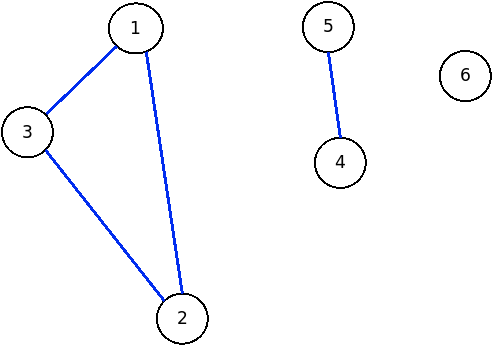
\includegraphics[width=\columnwidth]{img/patching1.png}
		\caption{The \texttt{single\_patch} input instance.}
		\label{fig:patching1}
	\end{subfigure}
\hfill%
	\begin{subfigure}{.26\columnwidth}
		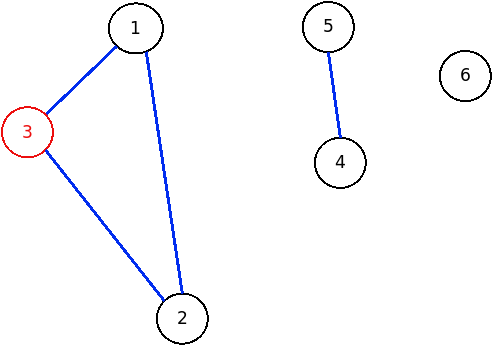
\includegraphics[width=\columnwidth]{img/patching2.png}
		\caption{Node $ 3 $ is chosen randomly from a set of subtours.}
		\label{fig:patching2}
	\end{subfigure}
\hfill%
	\begin{subfigure}{.26\columnwidth}
		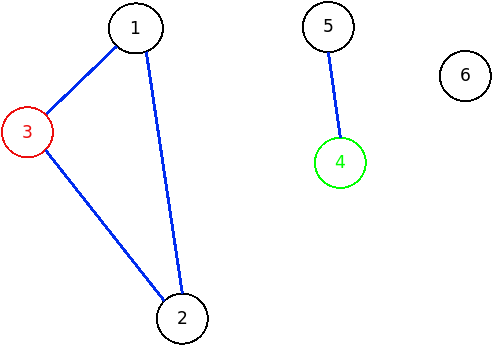
\includegraphics[width=\columnwidth]{img/patching3.png}
		\caption{It is selected the closer node to $ 3 $ which is in a different tour (node $ 4 $).}
		\label{fig:patching3}
	\end{subfigure}
	\begin{subfigure}{.26\columnwidth}
		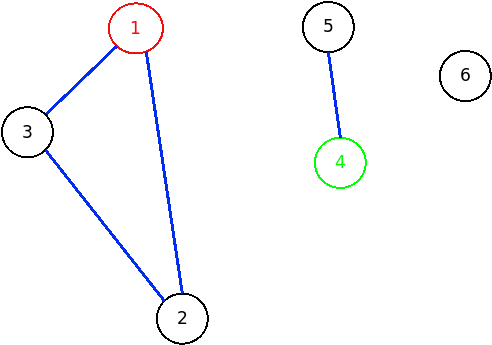
\includegraphics[width=\columnwidth]{img/patching4.png}
		\caption{Iterating throw the first tour nodes, it is selected the node which minimize the next merge cost.}
		\label{fig:patching4}
	\end{subfigure}
\hfill%
	\begin{subfigure}{.26\columnwidth}
		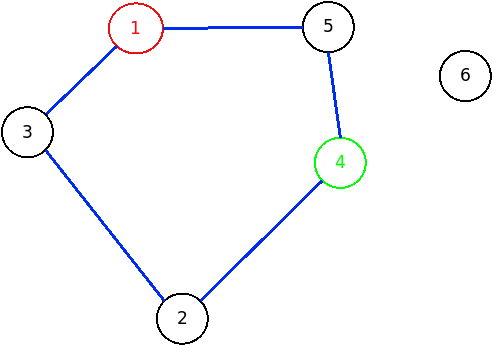
\includegraphics[width=\columnwidth]{img/patching5.png}
		\caption{Merge operation.}
		\label{fig:patching5}
	\end{subfigure}
\hfill%
	\begin{subfigure}{.26\columnwidth}
		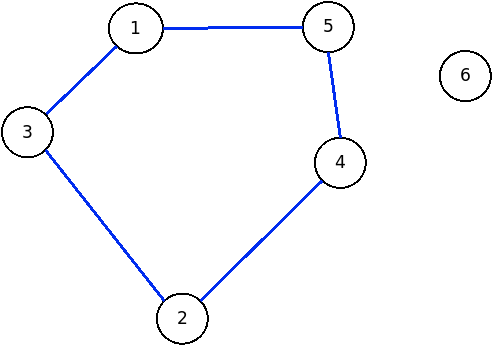
\includegraphics[width=\columnwidth]{img/patching6.png}
		\caption{The final result.}
		\label{fig:patching6}
	\end{subfigure}
\caption{Single patch move algorithm}
\label{fig:single_patch}
\end{figure}\\
A \texttt{succ} structure is use to represent the input tours, which for each  $ i = 1, .., n = |V|$ is defined as: 
\begin{equation}
\texttt{succ[i] = } \begin{cases}
 \text{"\texttt{i} successor"} & \text{if \texttt{i} is in a tour,}\\
 \text{\texttt{-1}} & \text{otherwise.}
\end{cases}
\end{equation} \\
In the \texttt{succ} structure, each edge could be considered as oriented: if \texttt{succ[i] = j} than \texttt{i} $\rightarrow$ \texttt{j} is the considered edge orientation. \\
The merge phase is the core of the method. To avoid a large number of intersection between edges, which is a sign of non optimal solution, all the tour are initialize in clockwise orientation and the merge phase must keep the property in the output tour. An example of merge is done in fig \ref{fig:patching_merge}. Note that once the two nodes are selected there are only two possible merge: one create the intersection and the other one does not. It is easy to prove that without intersection the tour is shorter. Moreover if each tour is clockwise, the property is naturally maintained
\begin{figure}[!h]
	\begin{subfigure}{.26\columnwidth}
		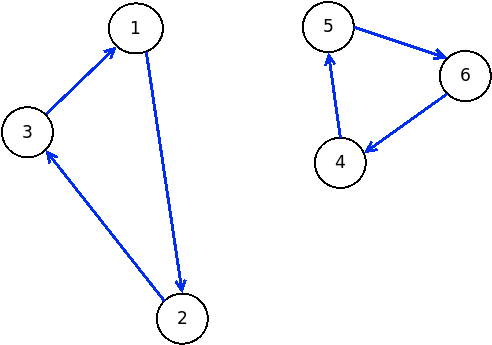
\includegraphics[width=\columnwidth]{img/patching_merge1.png}
		\caption{}
		\label{fig:patching_merge1}
	\end{subfigure}
	\hfill%
	\begin{subfigure}{.26\columnwidth}
		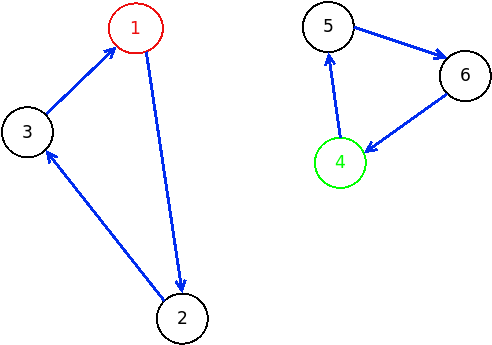
\includegraphics[width=\columnwidth]{img/patching_merge2.png}
		\caption{}
		\label{fig:patching_merge2}
	\end{subfigure}
	\hfill%
	\begin{subfigure}{.26\columnwidth}
		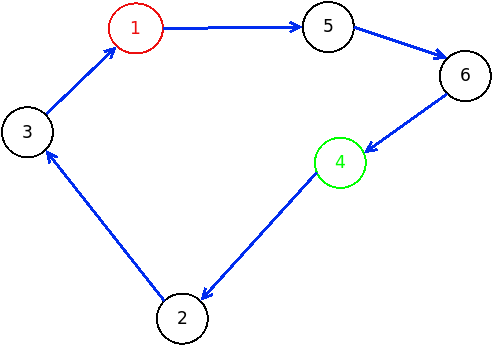
\includegraphics[width=\columnwidth]{img/patching_merge3.png}
		\caption{}
		\label{fig:patching_merge3}
	\end{subfigure}

	\caption{Merge phase in detail. Note that the orientation of the arch is that expressed from the associated \texttt{succ} structure, however the problem is aTSP, therefore the edges are not oriented.}
	\label{fig:patching_merge}
\end{figure}\\

\begin{table}[h]
	\centering
	\caption{The \texttt{succ} structure for the tour in figure \ref{fig:patching_merge}}
	\begin{tabular}{clcccccc}
		\multirow{2}{*}{\ref{fig:patching_merge1})} 	& \texttt{i:}		& 1 & 2 & 3 & 4 & 5 & 6 \\
														& \texttt{succ[i]:}	& 2 & 3 & 1 & 5 & 6 & 4 \\
														&		   			&   &   &   &   &   &   \\
		\multirow{2}{*}{\ref{fig:patching_merge3})} 	& \texttt{i:}		& 1 & 2 & 3 & 4 & 5 & 6 \\
														& \texttt{succ[i]:}	& 5 & 3 & 1 & 2 & 6 & 4 \\
	\end{tabular}
\end{table}
To keep the clockwise orientation of the tour there is a special consideration have to be done to merge an isolated node with a tour of two nodes. In the final tour the clockwise property must is checked if the condition is satisfied:
$ (x_3 - x_1)*(y_2 - y_1) < (y_3 - y_1)*(x_2 - x_1) $,
otherwise the tour is reversed.
\begin{figure}[!h]
	\centering
	\begin{subfigure}{.2\columnwidth}
		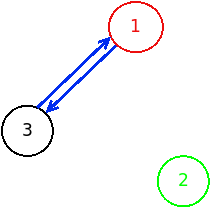
\includegraphics[width=\columnwidth]{img/patching_merge_clockwise1.png}
		\caption{Tours to be merged}
		\label{fig:patching_merge_clockwise1}
	\end{subfigure}
\hfill
	\begin{subfigure}{.46\columnwidth}
		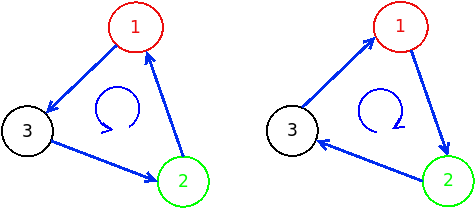
\includegraphics[width=\columnwidth]{img/patching_merge_clockwise2.png}
		\caption{Two different orientation can result with the same cost. The clockwise orientation is accepted, otherwise the tour is reversed.}
		\label{fig:patching_merge_clockwise2}
	\end{subfigure}
	\caption{Special case of merge phase that create a tour with 3 edges. The orientation of the tour must be reverse if necessary.}
	\label{fig:patching_merge_clockwise}
\end{figure}
